% typ dokumentu
\documentclass[12pt,twoside]{article}

% użycie pakietu , jak include
\usepackage{weiiszablon}

% autor pracy
\author{Krystian Olszowy}

% np. EF-123456, EN-654321, ..., Numer albumu
\studentID{EA-167582}

\title{Tworzenie drzewa składniowego języka ST}
\titleEN{{Creating an ST language syntax tree}}


%%% wybierz rodzaj pracy wpisując jeden z poniższych numerów: ...
% 1 = inżynierska	% BSc
% 2 = magisterska	% MSc
% 3 = doktorska		% PhD
%%% na miejsce zera w linijce poniżej
\newcommand{\rodzajPracyNo}{2}


%%% promotor
\supervisor{dr inż. Jan Sadolewski}
%% przykład: dr hab. inż. Józef Nowak, prof. PRz

%%% promotor ze stopniami naukowymi po angielsku
\supervisorEN{Jan Sadolewski, PhD, Eng.}


%% DO ZROBIENIA %%
\abstract{Praca zawiera zaproponowane rozwiązanie sterowania telewizorem z poziomu smartfona dzięki aplikacji mobilnej i urządzeniu pośredniczącemu, opartemu o mikrokontroler z niezbędnymi modułami. Przedstawiono i omówiono w niej technologie i koncepty, z których korzystano podczas procesu projektowania i tworzenia rozwiązania. Opisane zostały też najważniejsze elementy fizycznej części systemu, oprogramowanie mikrokontrolera, zbudowana aplikacja mobilna oraz ich współpraca w celu sterowania urządzeniem telewizyjnym.}
\abstractEN{The work encompasses a solution for television control through a smartphone application and an intermediary device, based on a microcontroller with necessary modules. It introduces and discusses the technologies and concepts employed during the design and building process. Additionally, it details the key components of the physical system, microcontroller software, the developed mobile application, and their collaboration for television device control.}

%% DO ZROBIENIA %%
\keywords{ST language, syntax tree, CPDev, Flutter, aplikacja mobilna}
\keywordsEN{remote controller, BLE, IR, Flutter, mobile application}


\begin{document}

% strona tytułowa
\maketitle

\blankpage

% spis treści
\tableofcontents

\clearpage
\blankpage

\section{Wstęp}
\subsection{Zintegrowane środowiska programistyczne (ang. IDE)}
Współczesny inżynier czy programista automatyki nie wyobraża sobie pracy bez dostępu do zintegrowanego środowiska programistycznego (ang. IDE). Środowiska te, będące podstawowym narzędziem w pracy twórców oprogramowania sterowników PLC, przekształciły się z prostych edytorów kodu w zaawansowane platformy wspierające projektowanie, symulację, testowanie i wdrażanie systemów sterowania. Dzięki nim możliwe jest nie tylko wygodne tworzenie logiki sterującej, ale również wizualizacja procesów, zarządzanie konfiguracją sprzętu czy analizowanie działania programu w~czasie rzeczywistym.

Na rynku dostępnych jest wiele rozwiązań, różniących się zakresem funkcji, kompatybilnością z określonymi typami sterowników oraz poziomem zaawansowania użytkownika. Jednym z przykładów takiego środowiska jest CPDev - polskie oprogramowanie tworzone na Politechnice Rzeszowskiej wspierające języki programowania zgodne z normą IEC 61131-3, które umożliwia programowanie sterowników różnych producentów, symulację działania programu oraz jego późniejsze wdrożenie na urządzeniu docelowym. Choć wiele firm korzysta z komercyjnych środowisk oferowanych przez producentów sterowników, takich jak TIA Portal czy GX Works, to rosnąca popularność rozwiązań niezależnych - jak CPDev - pokazuje, że możliwe jest tworzenie otwartych, elastycznych i konkurencyjnych narzędzi dla branży automatyki.

\subsection{Drzewa składniowe}
Drzewa składniowe to jedno z tych narzędzi, które trudno przecenić w świecie programowania. Choć na pierwszy rzut oka mogą wydawać się technicznym detalem, w~praktyce są fundamentem działania wielu elementów środowisk programistycznych. To właśnie one przedstawiają kod w postaci uporządkowanej struktury, zgodnej z gramatyką danego języka, dzięki czemu program może być łatwiej analizowany i przetwarzany.

Bez drzew składniowych trudno wyobrazić sobie działanie kompilatorów, interpreterów, a nawet tak podstawowych funkcji edytora jak kolorowanie składni, podpowiadanie składniowe czy automatyczne formatowanie kodu. Dzisiejsze IDE bazują na tych strukturach niemal na każdym kroku - to one pozwalają na bieżąco wykrywać błędy w kodzie, usprawniają nawigację po projekcie i umożliwiają wprowadzenie inteligentnych podpowiedzi.

Automatyczne generowanie parserów, znacząco przyspiesza cały proces. Programista nie musi już ręcznie tworzyć złożonych analizatorów składni, co oszczędza czas i~ogranicza liczbę błędów.

Dla środowiska CPDev możliwość wygenerowania drzewa składniowego dla języka ST to istotne ułatwienie. Dzięki temu można nie tylko szybciej i prościej zaimplementować parser zgodny z normą IEC 61131-3, ale też stworzyć solidną podstawę do rozwijania edytora o nowe funkcje - jak choćby inteligentne podpowiedzi, analiza semantyczna czy lepsza diagnostyka błędów. To wszystko przekłada się na wygodniejszą pracę użytkownika i otwiera drogę do dalszego rozwoju CPDeva jako nowoczesnego narzędzia do programowania sterowników.


\subsection{Cel pracy}
Celem pracy jest przygotowanie interpretera kodu generującego drzewo składniowe języka ST zgodnego z normą IEC 61131-3 oraz oprogramowaniem CPDev, na~podstawie podanego kodu źródłowego tego języka. Oprogramowanie generujące drzewo składniowe ma współpracować z kodem w języku C\#. Aby takie oprogramowanie przygotować, należy wcześniej także przeprowadzić badanie porównawcze narzędzi do tworzenia drzew składni języków formalnych opisanych za pomocą gramatyki bezkontekstowej i wybrać rozwiązanie najbardziej odpowiadające postawionemu zadaniu.

\subsection{Zakres pracy}
Zakres pracy obejmuje prównanie wybranych narzędzi do tworzenia drzew skła\-dni języków formalnych opisanych za pomocą gramatyki bezkontekstowej i wybranie najlepszego z nich do interpretowania języka ST zgodnego z normą IEC 61131-3 w~CPDevie. Praca podejmuje także tematykę utworzenia pliku gramatyki języka ST dla najbardziej odpowiedniego z analizowanych narzędzi i przetestowania wygenerowanego oprogramowania dla przykładowych kodów źródłowych.


\subsection{Zawartość pracy DO ZROBIENIA}
W rozdziale drugim  omówiono ogólnodostępne rozwiązania stanowiące aktualny stan wiedzy w zakresie zdalnego sterowania odbiornikiem telewizyjnym. Prównano je z autorskim systemem wskazując jego zalety i rozwiązywane przez niego problemy.

Rozdział trzeci zawiera przedstawienie i opis technologii wykorzystanych w zaprojektowanym rozwiązaniu. Są to: Platforma ESP32, język programowania C++, framework Arduino, podczerwień, system Android, język programowania Dart, framework Flutter oraz techonlogia Bluetooth Low Energy.

Czwarty rozdział opisuje sposób połączenia komponentów składających się na urządzenie pośredniczące zbudowane aby skomunikować aplikację mobilną z telewizorem. Zawarte zostały w nim także opisane scharakteryzowane parametry tych komponentów.

W rozdziale piątym szczegółowo omówiono utworzone oprogramowanie mikrokontrolera odpowiedzialne za sterowanie jego zasobami i dołączonymi modułami fizyczymi. Przedstawione zostały ważniejsze kody źródłowe projektu oraz ich działanie.

Rozdział szósty zawiera opis zaprojektowanego intefejsu użytkownika aplikacji mobilnej oraz jej funkcjonalności. Ukazane zostały także wykorzystane podczas implementacji, rozwiązania programowe.

Siódmy rozdział koncentruje się na przedstawieniu sposobu korzystania z utworzonego rozwiązania. Dokonywana jest także ocena skuteczności działania poszczególnych funkcji systemu.

W ostatnim rozdziale zawarto podsumowanie całej pracy, możliwe usprawnienia zaprojektowanego rozwiązania. Wskazane zostały też elementy projektu, które autor uważa za wkład własny.


\clearpage
\section{Środowisko CPDev}
\subsection{Charakterystyka narzędzia}
CPDev (Control Program Developer) to otwarte, uniwersalne środowisko inżynierskie przeznaczone do tworzenia i wdrażania oprogramowania sterującego dla systemów automatyki. Powstało jako efekt wieloletnich prac badawczych i rozwojowych prowadzonych na Politechnice Rzeszowskiej. Głównym założeniem projektowym CPDev było stworzenie platformy, która będzie nie tylko zgodna z normą IEC 61131-3, ale również łatwa do przeniesienia na różne platformy sprzętowe i dostępna dla inżynierów oraz studentów jako narzędzie zarówno edukacyjne, jak i przemysłowe.

Jednym z głównych atutów CPDev jest modularność oraz szeroki zakres funkcjonalności obejmujący cały proces tworzenia aplikacji sterujących. Środowisko udostępnia zestaw edytorów tekstowych i graficznych, narzędzia do konfiguracji systemu, symulator sterownika oraz narzędzia do projektowania interfejsów HMI. Dzięki temu możliwe jest kompleksowe projektowanie i testowanie systemów sterowania bez konieczności stosowania zewnętrznych narzędzi.

Ważną cechą CPDev jest jego niezależność sprzętowa, osiągnięta dzięki zastosowaniu warstwy pośredniej w postaci wirtualnej maszyny, która interpretuje kod pośredni generowany przez kompilator. Takie podejście umożliwia łatwe wdrażanie systemu na różnych urządzeniach, w tym na mikrokontrolerach, procesorach ARM, a nawet na implementacjach FPGA. Jednocześnie zapewnia ono jednolity sposób działania aplikacji niezależnie od platformy sprzętowej.

Środowisko CPDev jest stale rozwijane i udoskonalane. W kolejnych wersjach wprowadzano m.in. wsparcie dla języków graficznych, rozszerzenia dla systemów wielordzeniowych, interfejsy XML pozwalające na współpracę z innymi narzędziami inżynierskimi oraz rozwiązania umożliwiające projektowanie zgodnie z podejściem MDD (Model-Driven Development). CPDev znalazł już zastosowanie w wielu wdrożeniach przemysłowych — zarówno w kraju, jak i za granicą.

Z punktu widzenia użytkownika, środowisko CPDev oferuje funkcjonalności znane z komercyjnych rozwiązań, przy czym wyróżnia się większą otwartością, możliwością adaptacji do konkretnych potrzeb oraz dostępnością szczegółów implementacyjnych. To wszystko sprawia, że CPDev stanowi atrakcyjną alternatywę wobec zamkniętych środowisk oferowanych przez producentów sprzętu automatyki.
\subsection{Programowanie za pomocą CPDev-a}
\subsubsection{Ogólny sposób korzystania z narzędzia}
Programowanie w środowisku CPDev odbywa się w ramach graficznego interfejsu IDE, które integruje różne etapy projektowania systemu automatyki: od pisania kodu sterującego, przez konfigurację sprzętu i symulację, aż po wdrożenie na urządzenie docelowe. Proces ten można podzielić na kilka etapów:

Tworzenie projektu - użytkownik definiuje strukturę programu, dodaje nowe jednostki organizacyjne (POUs), deklaruje zmienne globalne i lokalne.

Kodowanie logiki sterowania - za pomocą jednego lub kilku języków normy IEC 61131-3.

Konfiguracja sprzętu i zmiennych wejściowo-wyjściowych - z użyciem narzędzia CPCon.

Symulacja i testowanie - możliwa dzięki narzędziu CPSim, które pozwala uruchomić aplikację sterującą w trybie offline.

Generowanie kodu pośredniego (VMASM) - po kompilacji, aplikacja może zostać załadowana do wirtualnej maszyny uruchamianej na docelowym sterowniku.

\subsubsection{Dostępne języki programowania}
CPDev wspiera wszystkie języki określone w normie IEC 61131‑3, co pozwala użytkownikom wybrać najbardziej odpowiedni sposób definiowania logiki sterującej w zależności od specyfiki projektu lub preferencji osobistych.

a) ST (Structured Text)
Język ST jest tekstowym językiem wysokiego poziomu, przypominającym składnią Pascala lub języki z rodziny C. Oferuje bogaty zestaw struktur sterujących (pętle, warunki, bloki), obsługę typów prostych i złożonych oraz wyrażeń logicznych i arytmetycznych. CPDev umożliwia pisanie całych aplikacji w ST, a także używanie go do definiowania funkcji i bloków funkcyjnych.

b) IL (Instruction List)
IL to język niskopoziomowy, przypominający asembler. Umożliwia precyzyjne określanie instrukcji operujących na rejestrach i zmiennych. Jego stosowanie w CPDev jest obecnie rzadsze, ponieważ został wycofany z najnowszej wersji normy IEC 61131-3, ale nadal pozostaje dostępny dla kompatybilności.

c) FBD (Function Block Diagram)
FBD jest językiem graficznym, który pozwala na tworzenie logiki poprzez łączenie bloków funkcyjnych w sposób przypominający schematy blokowe. Jest chętnie wykorzystywany przez inżynierów o mniejszym doświadczeniu programistycznym, szczególnie w przemyśle.

d) LD (Ladder Diagram)
LD, znany także jako język drabinkowy, to język graficzny inspirowany schematami przekaźnikowymi. Ułatwia migrację klasycznych systemów sterowania przekaźnikowego do programowalnych sterowników PLC. CPDev umożliwia tworzenie programów w LD i konwersję do ST.

e) SFC (Sequential Function Chart)
SFC jest językiem służącym do modelowania logiki sekwencyjnej. Program składa się z kroków, przejść i warunków przejścia. W CPDev sekwencyjna struktura tworzona jest graficznie, a logika kroków i przejść może być zapisana w ST lub FBD.
\subsection{Implementacja CPDeva i architektura maszyny wirtualnej}
Implementacja środowiska CPDev została oparta na założeniu, że system sterowania powinien być niezależny od konkretnej platformy sprzętowej, a zarazem możliwy do wdrożenia w rzeczywistych aplikacjach przemysłowych. Aby to osiągnąć, architektura CPDev została podzielona na dwa główne poziomy: środowisko deweloperskie (IDE) oraz maszynę wirtualną (VM), która wykonuje wygenerowany program sterujący.

Środowisko deweloperskie
IDE CPDev zostało zaimplementowane w języku C\# na platformę .NET, co zapewnia nowoczesny interfejs graficzny, wygodę użytkowania i łatwość dalszej rozbudowy. Składa się z modularnych komponentów, takich jak edytory kodu źródłowego, narzędzia konfiguracyjne, symulatory, analizatory błędów i generator kodu pośredniego. Zastosowanie C\# i środowiska .NET pozwala na integrację z innymi narzędziami, obsługę graficznych języków programowania oraz wprowadzanie rozwiązań typowych dla nowoczesnych aplikacji okienkowych (GUI).

Kluczowym elementem działania środowiska jest kompilator, który tłumaczy kod źródłowy napisany w językach normy IEC 61131‑3 (głównie ST) do VMASM – pośredniego kodu niskiego poziomu wykonywanego przez maszynę wirtualną.

Maszyna wirtualna (VM)
Maszyna wirtualna CPDev to lekki, niezależny od sprzętu interpreter kodu VMASM, implementowany głównie w języku ANSI C, co zapewnia wysoką przenośność. Dzięki temu może ona działać na wielu różnych platformach sprzętowych, w tym na mikrokontrolerach (np. AVR, ARM), systemach wbudowanych (np. Raspberry Pi, STM32), a także w symulacji na komputerze PC.

Główne cechy maszyny wirtualnej CPDev:

Interpretacja kodu pośredniego – wykonywanie instrukcji zdefiniowanych w języku VMASM, które odpowiadają operacjom sterowania, przetwarzania danych, wywołań funkcji, obsługi zmiennych i struktur danych.

Obsługa standardowych typów danych – BOOL, INT, REAL, TIME, DATE, STRING, ARRAY, STRUCT itd.

Zarządzanie cyklicznym wykonywaniem programu sterującego – logika sterowania wykonywana jest w pętli cyklicznej, zgodnie z zasadami działania typowego sterownika PLC.

Zgodność z IEC 61131‑3 – pełne wsparcie dla elementów programistycznych normy, w tym POU (Program Organization Units), czyli programów, funkcji i bloków funkcyjnych.

Łatwa integracja – dzięki modularności i lekkiej strukturze możliwa jest łatwa integracja VM z innymi systemami, np. przez protokoły komunikacyjne lub interfejsy HMI.

Dodatkowo, maszyna wirtualna posiada także wersję uruchamianą bezpośrednio w systemie Windows, wykorzystywaną przez symulator CPSim, który umożliwia testowanie aplikacji sterujących bez konieczności posiadania fizycznego sterownika.

Architektura ogólna
Architektura CPDev zakłada wyraźny podział odpowiedzialności:

IDE (C\#/.NET)	Edycja kodu, analiza, konfiguracja, generowanie VMASM
VMASM (pośredni język)	Przenośna reprezentacja logiki sterującej
VM (ANSI C)	Wykonywanie kodu sterującego niezależnie od platformy

Takie podejście pozwala rozdzielić rozwój środowiska programistycznego od rozwoju platform sprzętowych oraz zachować pełną kompatybilność i kontrolę nad działaniem systemu na różnych poziomach.
\clearpage

\section{Drzewa składniowe na podstawie gramatyki bezkontekstowej}
\subsection{Wprowadzenie do gramatyk bezkontekstowych}
Gramatyka bezkontekstowa (CFG, context-free grammar) to matematyczny model służący do opisu struktury formalnych języków, takich jak języki programowania. Składa się z:
skończonego zbioru nieterminali (zmiennych),
zbioru terminali (symboli końcowych, np. słów kluczowych, operatorów),
zestawu produkcyjnych reguł, w których każdy nieterminal może być zastąpiony ciągiem terminali i/nieterminali,
specjalnego symbolu startowego.
Gramatyki bezkontekstowe są wystarczająco wyraźne, by opisać większość języków programowania (np. ST), ale jednocześnie na tyle proste, by dawać się wydajnie parsować algorytmicznie.

\subsection{Drzewa składniowe}
Drzewo składniowe to uporządkowana struktura w postaci drzewa, która wizualnie i strukturalnie odwzorowuje sposób, w jaki ciąg symboli terminalnych (np. kod programu) został wygenerowany przez gramatykę.

Korzeń drzewa to symbol startowy.

Węzły wewnętrzne reprezentują nieterminale.

Liście odpowiadają terminalom (lub czasem symbolowi pustemu)

Drzewo powstaje podczas parsowania: każda reguła produkcji zamienia nieterminal na jego dzieci w drzewie. Po lewej–prawej kolejności liści odczytujemy oryginalny ciąg słów, czyli kod źródłowy .

Drzewo składniowe służy jako:

Mapowanie struktury kodu (np. wyrażeń, instrukcji).

Podstawa analiz semantycznych, jak sprawdzanie typów.

Podstawowy model do generacji dalszego kodu (astrakcja, optymalizacja).

\subsection{Zastosowanie parserów w IDE i narzędziach}
W środowiskach takich jak CPDev parser generowany na podstawie gramatyki:
umożliwia kolorowanie składni, podpowiedzi, autokompletację;
wykrywa błędy już podczas pisania;
wspiera refaktoryzację kodu i zabezpiecza przekształcenia kodu;
dostarcza podstawę do generacji kodu pośredniego (e.g. VMASM).
\clearpage

\section{Przegląd narzędzi do automatycznego generowania drzew składni}
\subsection{Bison}
\subsection{Irony.Net}
\subsection{ANTLRv4}
\subsection{Porównanie}
\clearpage
\section{Utworzenie parsera języka ST przy pomocy ANTLRv4}
\subsection{Przygotowanie środowiska i utworzenie struktury projektu}
\subsection{Gramatyka - lexer}
\subsection{Gramatyka - parser}
\subsection{Ocena przygotowanego oprogamowania}
\clearpage
\section{Zakończenie}
\clearpage
\section{Urządzenie wysyłające sygnały IR}
\subsection{Schemat elektryczny zaprojektowanego urządzenia}
Aby wykonać urzadzenie pośredniczące najpierw wykonano shemat elektryczny przy pomocy programu EasyEDA w darmowej wersji online\cite{easyEda}. Dzięki bibliotekom tworzonym przez użytkowników odnaleziono wszystkie niezbędne elementy do działania urządzenia pośredniczącego. Utworzony schemat elektryczny powstały z użytych komponentów znajduje się na rysunku \ref*{Fig:deviceScheme}.
\begin{figure}[ht]
   \centering
   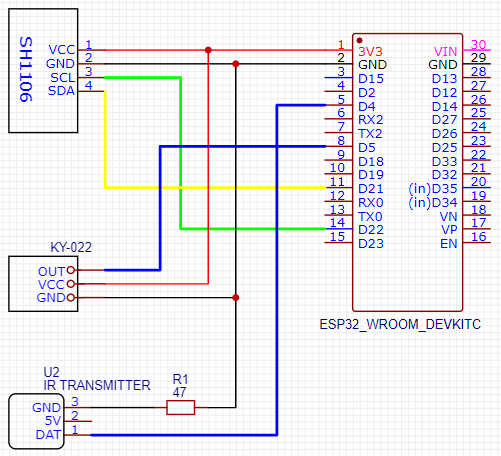
\includegraphics[width=12cm]{images/deviceScheme.png}
   \caption{Schemat elektryczny urządzenia pośredniczącego}
   \label{Fig:deviceScheme}
\end{figure}

Na schemacie kolorem czarnym oznaczono połączenia do masy (GND), kolorem czerwonym zasilanie z mikrokontrolera o potencjale 3.3 V. Na niebiesko zaznaczone są szyny danych modułów IR. Z kolei kolorem zielonym oznaczono linię zegarową, a~żółtym linię danych, porotokołu komunikacjynego I2C wyświetlacza OLED.

Samo urządznie nie jest wrażliwe na zakłócenia elektromagnetyczne, ani nie wymagało ochronnej obudowy do przestestowania poprawności założeń projektowych oraz końcowych testów pełnego systemu, dlatego jako element łączący moduły została użyta płytka stykowa. Dzięki użyciu płytki zachowano pełną funkcjonalność urządzenia oraz zyskano dowolność zmian podczas projektowania rozmieszczenia i połączenia komponentów. Urządznie osadzone na płytce prototypowej zostało przedstawione na rysunku \ref*{Fig:deviceOnBoard}.
\begin{figure}[ht]
   \centering
   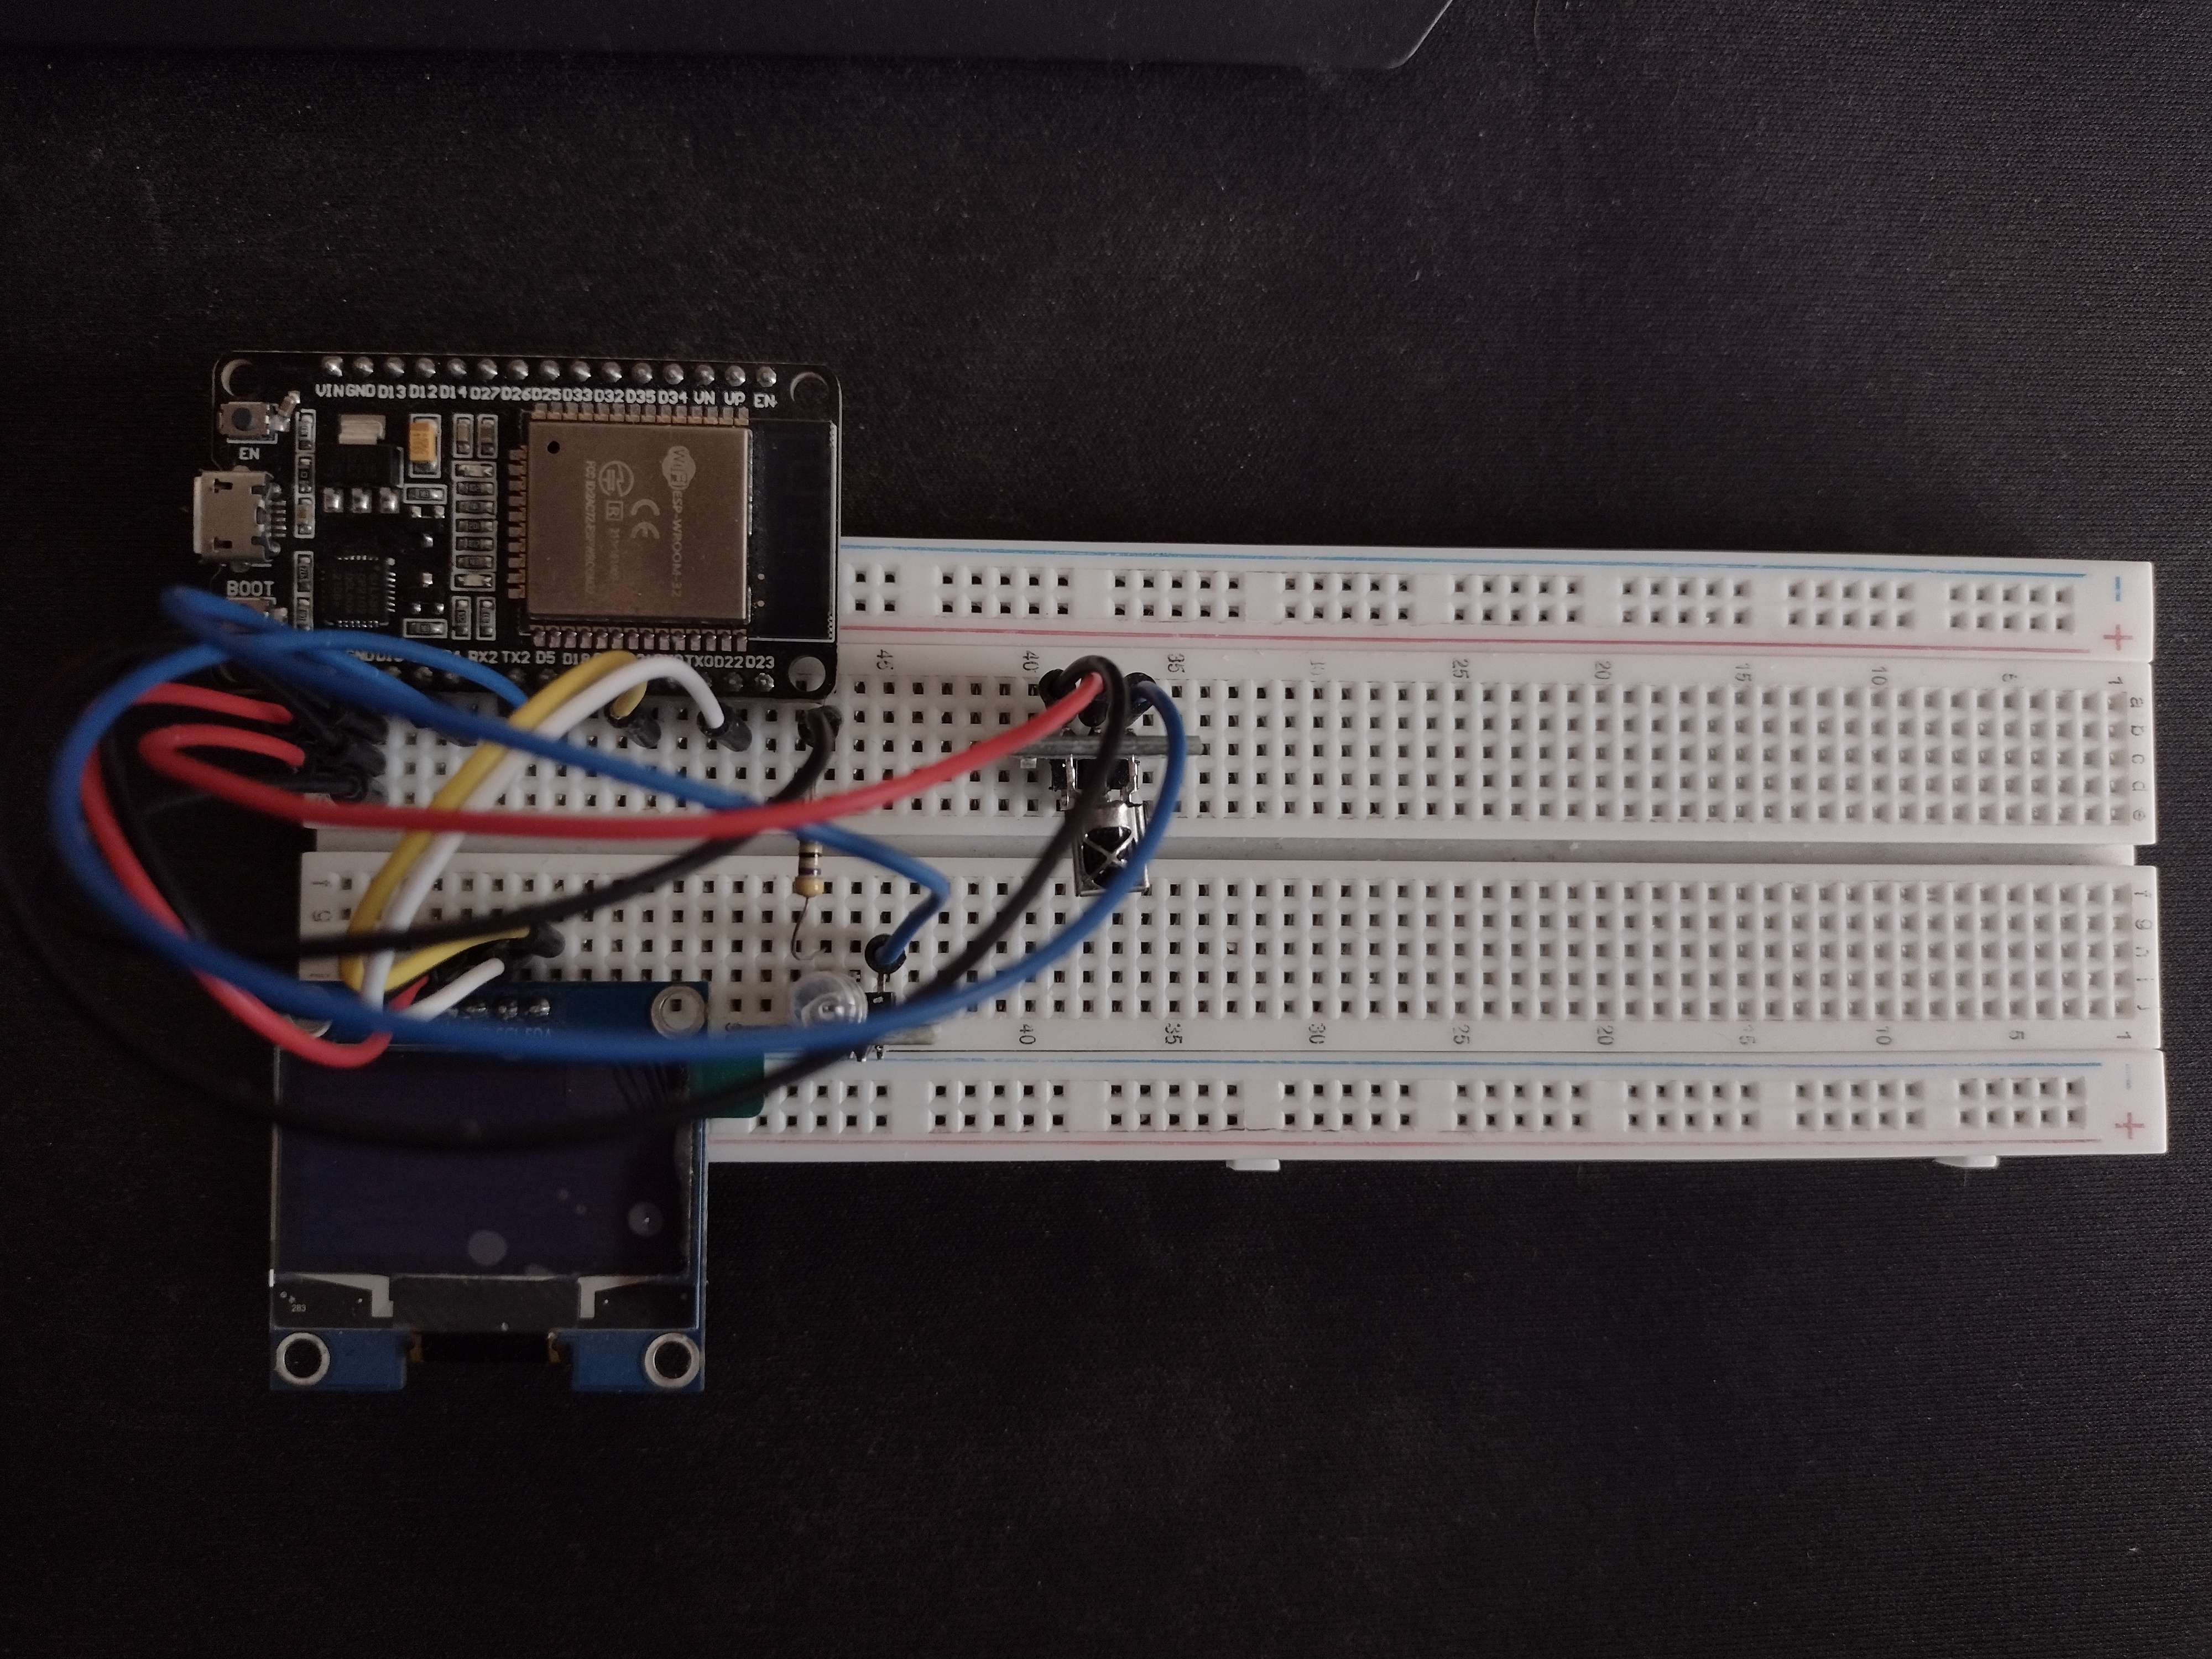
\includegraphics[width=12cm]{images/deviceOnBoard.jpg}
   \caption{Urządzenie pośredniczące osadzone na płytce prototypowej}
   \label{Fig:deviceOnBoard}
\end{figure}
\subsection{Przeglad i opis uzytych komponentow}
Elementy przedstawione na schemacie elektrycznym znalazły się w przedstawionym wcześniej modelu modelu fizycznym. Są to:
\begin{enumerate}[label=\alph*), leftmargin=1.25cm]
   \item Zestaw deweloperski ESP32 Wroom DevKitC V1\cite{doitDevKitV1} -- to system z mikrokontroler ESP32 z procesorem Dual Core Tensilica LX6 240 MHz, pamięcią SRAM 520 KB i pamięcią flash 4 MB. Posiada wbudowane moduły WiFi 802.11 b/g/n oraz moduł Bluetooth Low Energy, dzięki którym nie trzeba dołączać osobnych modułów komunikacji bezprzewodowej. Znajduje się na nim 30 wyprowadzeń GPIO w postaci goldpinów, co znacznie zwiększa wygodę projektowania. Zasilany jest z 5 V ze złącza microUSB lub pinu VCC i GND.
   \item Wyświetlacz OLED SH1106\cite{sh1106} -- to wyświetlacz OLED o przekątnej 1,3'' i rozdzielczości 128 pikseli na 64 pikesle. Ekran oparty jest na sterowniku Adafruit SH1106 pracuje z napięciami 3,3 V oraz 5 V, komunikuje się poprzez protokół I2C. Posiada wlutowane proste złącza goldpin. Wyświetla znaki w kolorze białym.
   \item Transmiter IR KY-005\cite{ky005} -- to moduł nadawczy sygnałów podczerownych. Obsługuje wysyłanie fal IR o długości 940 nm. I pobiera 90 mW mocy podczas działania.
   \item Odbiornik IR KY-022\cite{ky022}  -- to moduł z odbiorczy podczerwieni, działający na częstotliwości 38 kHz. Zasilany jest napięciem od 2,7 V do 5,5 V. Wykrywa sygnał pod maksymalnym kątem odchylenia 90°. Maksymalna odległość wykrywania: 18 m. Posiada cyfrowy sygnał wyjściowy.
   \item Rezystor 47 Ohm -- resystor przewlekany o tolerancji 5 \% i makasymalnej mocy 0,25 W.
   \item Przewody połaczeniowe męsko-męskie.
   \item Płytka stykowa.
\end{enumerate}

\clearpage

\section{Oprogramowanie sterujące urządzeniem wysyłającym sygnały IR}
\subsection{Środowisko narzędziowe}
Kod sterujący urządzeniem pośredniczącym opartym o mikrokontroler ESP32 został przygotowany za pomocą jezyka C++ oraz frameworka Arduino. Cały projekt oprogramowania zarządzany był przez rozszerzenie do edytora tekstu Visual Studio Code czyli PlatformIO, przy pomocy którego, doinstalowywane były też wymagane biblioteki oraz budowany i wgrywany na płytkę ESP32 Wroom DevKitC był program sterujący, a także przeprowadzane debugowanie. Każda z tych operacji mogła się odbyć dzięki wsparciu programowania i debugowania za pomocą portu microUSB, które posiadała płytka oraz rozszerzenie edytora tekstu.
\subsection{Ogólna struktura oprogramowania}
Oprogramowanie sterujące urządzeniem wysyłąjącym sygnały podczerowne zostało podzielone na 4 elementy. Główny z nich to plik \kod{main.cpp} gdzie odbywa się sterowanie urządzeniem, korzystając przy tym z pozostałych modułów. Utworzone zostały 3 moduły narzędziowe, aby główny kod stał się bardziej przejrzysty oraz modularny. Opdowiadają one za obsługę wyświetlacza OLED, komunikację BLE oraz interpretację danych pochodzących z charakterystyk BLE. Wynikowa struktura podziału autorskich elementów oprogramowania została przedstawiona na rysunku \ref*{Fig:codeStructure}.
\begin{figure}[ht]
   \centering
   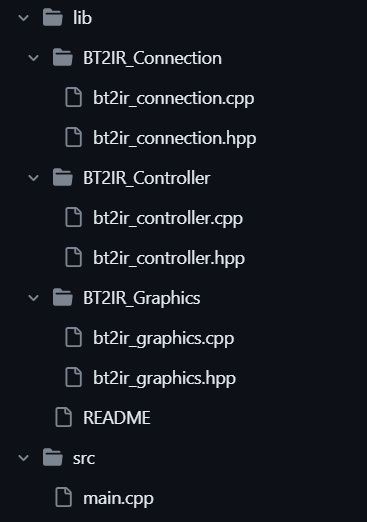
\includegraphics[width=4.5cm]{images/codeStructure.png}
   \caption{Struktura oprogramowania sterującego urządzeniem pośredniczącym}
   \label{Fig:codeStructure}
\end{figure}

\subsection{Główny program sterujący}
Główny program, który steruje całym urządzeniem pośredniczącym znajduje się w~pliku \kod{main.cpp}. Aby zorzumieć jakie funkcjonalności oferuje, najlepiej prześledzić jego budowę.

Najpierw dołączane są pliki nagłówkowe z frameworka Arduino dla ESP32 odpowiadające za obsługę wysyłu i odbioru syngałów podczerwonych. Dołączane są także autorskie moduły z przestrzeni nazw \kod{bt2ir}. Korzystając z nich z kolei można utworzyć globalne obiekty klas, które pozwalają na zarządzanie połączeniem BLE, interpretację danych z charakterystyk tego połączenia, i pracę z  wyświetlaczem OLED. Obiekty tych klas zostają zinicjowane odpowiednimi danymi, prawidłowymi dla posiadanego sprzętu, jak rozdzielczość ekranu OLED czy numery pinów płytki deweloperskiej, na których będą przesyłane dane z i do modułów IR. Kod realizujący dołączanie plików nagłówkowych oraz inicjalizację obiektów globalnych znajduje się na listingu \ref{Lst:globalDefinitions}.

\lstinputlisting[inputencoding=utf8/cp1250, language={C++}, caption={\protect\input{captions/globalDefinitions.txt}\protect\relax}, label={Lst:globalDefinitions}]{codes/globalDefinitions.cpp}

Framework Arduino oczekuje zedefiniowania funkcji \kod{setup()}, która będzie wykonywana raz podczas uruchomienia urządzenia. Utworzono takową i zawarto w niej już na początku zainicjowanie połaczenia szeregowego, aby móc odczytywać dane z~urządzenia, na wypadek chęci wykrycia błędów działania. Znalazła się tam także inicjacja połaczenia z wyświetlaczem OLED poprzez protokół I2C oraz inicjacja serwera BLE, obie inicjacje zostały przeprowadzone za pomocą metod obiektów klas z autorskich modułów. Rozpoczęto w tej funkcji już nasłuchiwanie sygnałów podczerwonych i zainicjowano pracę modułu wysyłającego sygnały IR przy pomocy wcześniej utworzonych obiektów. Zawartość funkcji \kod{setup()} przedstawia kod źródłówy na listingu \ref*{Lst:setup}.

\lstinputlisting[inputencoding=utf8/cp1250, language={C++}, caption={\protect\input{captions/setup.txt}\protect\relax}, label={Lst:setup}]{codes/setup.cpp}

Tworząc oprogramowanie za pomocą frameworka Arduino zdefiniować należy także funkcję, która będzie wykonywana w nieskończonej pętli na programowanym urządzeniu. Narzędzie wymaga nazywała się ona \kod{loop()}. Przed nią jednak znalazły się jeszcze inicjalizacje dwóch znaczników czasowych w postaci dodatnich liczb całkowitych, które zostaną użyte do odliczania czasu trwania wyświetlania komunikatów dla użytkownika.

\begin{figure}[!ht]
\lstinputlisting[inputencoding=utf8/cp1250, language={C++}, caption={\protect\input{captions/loop1.txt}\protect\relax}, label={Lst:loop1}]{codes/loop1.cpp}  
\end{figure}

W samej już funkcji umieszczono instrukcje warunkowe, przez które, sprawdzane jest czy wstąpiły zdarzenia, takie jak: odebranie danych za pomocą serwera BLE o wciśniętym klawiszu w aplikacji, odebranie sygnału podczerwonego na module odbiornika IR, czy też rozłączenie lub połączenie z serwerem BLE nowego użytkownika aplikacji mobilnej. Jeśli program wykryje zdarzenie serwera BLE, rysuje na wyświetlaczu OLED odświeżony stan połaczenia zwierający informację o liczbie połączonych użytkowników. Jeśli z kolei wykryte zostanie zdarzenie odebrania na serwerze BLE informacji o typie wciśniętego przycisku, rysowana jest jego ikona i nazwa, aby poinformować użytkownika o~otrzymaniu jego żądania. Po obsłużeniu zdarzenia resetowana jest flaga informująca o~jego aktywności. Obsługa opisanych zdarzeń w pierwszej części funkcji \kod{loop()} została przedstawiona na listingu \ref*{Lst:loop1}.


\begin{figure}[!ht]
\lstinputlisting[inputencoding=utf8/cp1250, language={C++}, caption={\protect\input{captions/loop2.txt}\protect\relax}, label={Lst:loop2}]{codes/loop2.cpp}
\end{figure}

Program reaguje też na otrzymanie szesnastkowego kodu IR po wciśnieciu przycisku  pilota w aplikacji mobilnej. Po otrzymaniu tego kodu przez BLE, przesyłany jest on dalej w formie sygnału podczerwonego do telewizora, realizując w ten sposób sterowanie nim, po zakończeniu już obsługi zdarzenia resetowana jest jego flaga. Jeżeli odczytany zostanie na zewnętrznym module odbiorczym, prawidłowy sygnał podczerwony, wypisany zostaje on na wyświetlaczu OLED, dzięki dedykowanej metodzie obiektu sterującego tym ekranem. Aktualizowany zostaje też wtedy znacznik czasowy tego zdarzenia. Następnie też wznawiane jest nasłuchiwanie sygnałów podczerwonych. Każdy z komunikatów dla użytkownika posiada swój czas wyświetlania. Limitowanie czasu ich trwania jest realizowane za pomocą sprawdzania stempli czasowych. Jeśli któryś z komunikatów powinien już się zakończyć, co jest wnioskowane na podstawie odległości aktualnego czasu od odpowiedniego znacznika czasowego, resetowane są wszystkie znaczniki czasowe komunikatów i następuje wyświetlenie domyślnego ekranu stanu połączenia BLE. Te funkcjonalności znalazły się w drugiej części funkcji \kod{loop()}, a jej kod źródłowy został przedstawiony na listingu \ref{Lst:loop2}.



\subsection{Moduł komunikacji poprzez BLE}
Autorski moduł odpowiedzialny za komunikację BLE został oparty o moduły biblioteki NimBLE\cite{nimBLE}, zamiast podstawowej biblioteki przygotowanej przez Arduino, ponieważ ta druga zajmowała zbyt wiele miejsca w pamięci FLASH mikrokontrolera. Wszystkie elementy tego modułu znalazły się w przestrzeni nazw \kod{bt2ir}.

Klasa zarządzająca połaczeniem BLE została utworzona przy pomocy wzorca projektowego Singleton\cite{designPatterns}, który powoduje że użytkownich korzysta z logicznie tylko jednej instancji takiej klasy, przechowywanej pomiędzy obiektami za pomocą uchywtu, którym dla języka C++ stał się wskaźnik. Zasosowano ten wzorzec aby zachowywać informacje o połączeniu BLE w całym programie i modduły mogły korzystać jednocześnie z tego samego połącznia w wygodny sposób. Publiczne funkcjonalności tej klasy udostępnione za pomocą metod to:
\begin{enumerate}[label=\alph*), leftmargin=1.25cm]
   \item inicjalizacja serwera BLE
   \item możliwość odczytywania i edytowania liczby połączonych urządzeń
   \item możliwość odczytywania i edytowania flag zdarzeń odebrania danych wciśniętego przycisku w aplikacji mobilnej
   \item dostęp do charakterystyk odebranego typu przycisku i jego kodu IR
   \item metoda pozwalająca narysować aktualny stan połączenia BLE.
\end{enumerate} Część pliku nagłówkowego zawierająca dostępne metody publiczne klasy \kod{Connection} została przedstawiona na listingu \ref*{Lst:bleMethods}.

\lstinputlisting[inputencoding=utf8/cp1250, language={C++}, caption={\protect\input{captions/bleMethods.txt}\protect\relax}, label={Lst:bleMethods}]{codes/bleMethods.cpp}

Najważniejszym elementem tego modułu jest metoda \kod{setupConnection()} klasy \kod{Connection}. W niej właśnie odbywa się inicjowanie serwera BLE wraz z jego parametrami oraz dołączenie funkcji wywoływanych podczas zdarzeń serwera.

Podczas przygotowywania urządzenia pośredniczącego do obsługi BLE w pierwszej kolejności inicjowane jest abstrakcja urządzenia. Kolejno dalej na urządzeniu tworzony jest serwer i przypisywane są mu autorskie klasy przechowujące metody wywoływane przez zdarzenia serwera, zawarte także w tym module, dzięki czemu biblioteka automatycznie będzie wykonywać czynności po połączeniu i rozłączeniu użytkownika, oraz o takim wydarzeniu zostanie poinformowany główny program sterujący.
Na tak utworzonym serwerze tworzony jest serwis i jego 2 charakterystyki odpowiadające wyłącznie za odbieranie danych o typie wciśniętego przycisku i jego szesnastkowym kodzie IR. Obie charakterystyki otrzymują także swoje klasy z metodami wywoływanymi podczas odebrania danych, dzięki czemu główny program sterujący informowany jest o tym zdarzeniu. Utworzony w ten sposób serwer może rozpocząć rozgłaszanie swojej obecności i nazwiązywać połączenia z klientami. Kod funkcji realizującej inicjalizację serwera BLE znajduje się na listingu \ref*{Lst:setupConnection}.

\lstinputlisting[inputencoding=utf8/cp1250, language={C++}, caption={\protect\input{captions/setupConnection.txt}\protect\relax}, label={Lst:setupConnection}]{codes/setupConnection.cpp}

Aby uzyskać możliwość połaczenia wielu użytkowników z serwerem BLE urządzenia pośredniczącego metoda wywoływana podczas każdego połączenia nowego użytkownika musi wznowić rozgłaszanie dostępności serwera. Ta funkcjonalność została zaimplementowana w funkcjach wywwoływanych podczas zdarzeń serwera.
\subsection{Moduł interpretujący dane z serwera BLE}
Aby ułatwić pracę z danymi odebranymi przez urządznie pośredniczące utworzono moduł przetwarzający je. Zawiera on wygodny typ wylieczniowy wykorzystywany do nadawania przejrzystych nazw programowych dla odebranych typów wciśniętego przycisku pilota z aplikacji mobilnej.
Z kolei klasa \kod{Controller} odpowiada za interpretację danych, odebranych za pomocą charakterystyk serwera BLE. Korzysta ona z instancji klasy \kod{Connection} aby pobrać dane z charakterystyk i je przetworzyć. W~tym celu, klasa ta, udostępnia metody pozwalające odświeżać przechowywane jej polach prywatnych ostatnio odebrane dane od aplikacji mobilnej. Publicznie dostępne elementy modułu znajdują się na listingu \ref*{Lst:controller}.
\vfill

\lstinputlisting[inputencoding=utf8/cp1250, language={C++}, caption={\protect\input{captions/controller.txt}\protect\relax}, label={Lst:controller}]{codes/controller.cpp}

Dane odebrane za pomocą charakterystyk przechowywane są w postaci bitowej. Aby odczytać ich wartości należy zinterpretować ich zawartość za pomocą odpowiedniego szablonu, który w tym przypadku będzie typem danych. Metoda \kod{updateButton\-Type()} z klasy \kod{Controller} interpretuje dane charakterystki za pomocą typu 8~bitowej liczby całkowitej bez znaku, ponieważ ilość przycisków jest niewielka. Odbywa się tam też prosta kontrola poprawności danych, poprzez sprawdzenie czy odebrane dane mieszczą się w zakresie zdefiniowanych przycisków pilota. Kod źródłowy tej funkcji znajduje się na listingu \ref*{Lst:dataProcessing}.

\lstinputlisting[inputencoding=utf8/cp1250, language={C++}, caption={\protect\input{captions/dataProcessing.txt}\protect\relax}, label={Lst:dataProcessing}]{codes/dataProcessing.cpp}

\subsection{Moduł obsługi ekranu OLED}
Autorski moduł obsługi ekranu OLED jest w rzeczywistości nakładką na klasę sterującą wyświetlaczem OLED z bibliotek firmy Adafruit. Taka relacja realizowania jest za pomocą dziedziczenia publicznego po klasie \kod{Adafruit\_SH1106G} w utworzonej klasie nakładki \kod{Display}. Sama nakładka znalazła się w przestrzeni nazw \kod{bt2ir}.

Utworzona klasa nakładki stara się udostępnić metody, dzięki którym użytkownik w prosty i przejrzysty sposób może rysować konkretne obrazy i napisy na wyświetlaczu, w postaci przygotowanych i zparametryzowanych ekranów. Udostępnione zostały ekrany takie jak przedstawienie liczby połączonych smartfonów z serwerem BLE i jego stanu, wyświetlanie komunikatu o odebraniu wciśniętego przycisku z aplikacji mobilnej, czy wyświetlenia odebranego za pomocą modułu odbiorczego z diodą sygnału IR. Lista dostępnych funkcjonalności utworzonej nakładki w postaci metod publicznych została przedstawiona na listingu \ref*{Lst:graphics}.

\lstinputlisting[inputencoding=utf8/cp1250, language={C++}, caption={\protect\input{captions/graphics.txt}\protect\relax}, label={Lst:graphics}]{codes/graphics.cpp}

Ukryta dla użtykownika logika tej nakładki opiera się o 4 metody prywatne. Dwie z nich rysują bardziej podstawowe elementy ekranów, takie jak rysowanie wyrównanego tekstu czy wielkich cyfr. Dzięki nim powstały także dwie metody z nich korzystające, przy pomocy których, można narysować na wyświetlaczu ikonę z podpisem lub cyfrę z podpisem. Tak wydzielone fragmenty logiki kodu, przyspieszyły i~ułatwiły zbudowanie wszystkich publicznie dostępnych funkcjonalności. Utworzona lista prywatnych metod zaprojektowanej klasy znajduje się na listingu \ref*{Lst:graphicsPrivate}.

\lstinputlisting[inputencoding=utf8/cp1250, language={C++}, caption={\protect\input{captions/graphicsPrivate.txt}\protect\relax}, label={Lst:graphicsPrivate}]{codes/graphicsPrivate.cpp}

Ikony rysowane na ekranach przez publiczne metody nakładki zostały umieszczone w programie za pomocą tablic bajtów, a same tablice zostały wygenerowane poprzez progowanie binarne obrazów w odcieniach szarości, przy pomocy aplikacji internetowej image2cpp\cite{image2cpp}. Po przekonwertowaniu obrazów na tablice bajtów i usunięciu z~jej otoczenia niepotrzebnie wygenerowanych części kodu, można ją umieścić w oprogramowaniu i wykorzystywać do wyświetlania obrazu, którego ta tablica dotyczy. Jedna z~wygenerowanych tablic znajduje się na listingu \ref*{Lst:imageArray}.
\vfill

\lstinputlisting[inputencoding=utf8/cp1250, language={C++}, caption={\protect\input{captions/imageArray.txt}\protect\relax}, label={Lst:imageArray}]{codes/imageArray.cpp}

Dzięki utworzonym narzędziom budowano publiczne metody dostępne dla użytkownika nakładki. W każdej takiej funkcji najpierw czyszczony był wyświetlacz, następnie rysowano w buforze ekranu odpowiedni obraz na podstawie zdefiniowanych tablic bajtów wraz z wyśrodkowanym podpisem, by końcowo wyświetlić dane zgromadzone w~buforze rysowania. Jedną z tych metod jest \kod{drawMoveUp()} rysująca komunikat dla użytkownika o wciśnięciu przycisku przejścia w górę na pilocie w aplikacji mobilnej. Jej implementacja została przedstawiona na listingu \ref*{Lst:drawMoveUp}, a jej fizyczny efekt na wyświetlaczu OLED pokazano na rysunku \ref*{Fig:drawMoveUp}.

\lstinputlisting[inputencoding=utf8/cp1250, language={C++}, caption={\protect\input{captions/drawMoveUp.txt}\protect\relax}, label={Lst:drawMoveUp}]{codes/drawMoveUp.cpp}

Więcej ekranów i obrazów, które może przedstawiać wyświetlacz OLED osadzony w urządzeniu pośredniczącym zostały zawarte w prezentacji pełnego systemu. W ten sposób opatrzone są w odpowiedni konekst ułatwiający zrozumienie ich celowości.

\begin{figure}[ht]
   \centering
   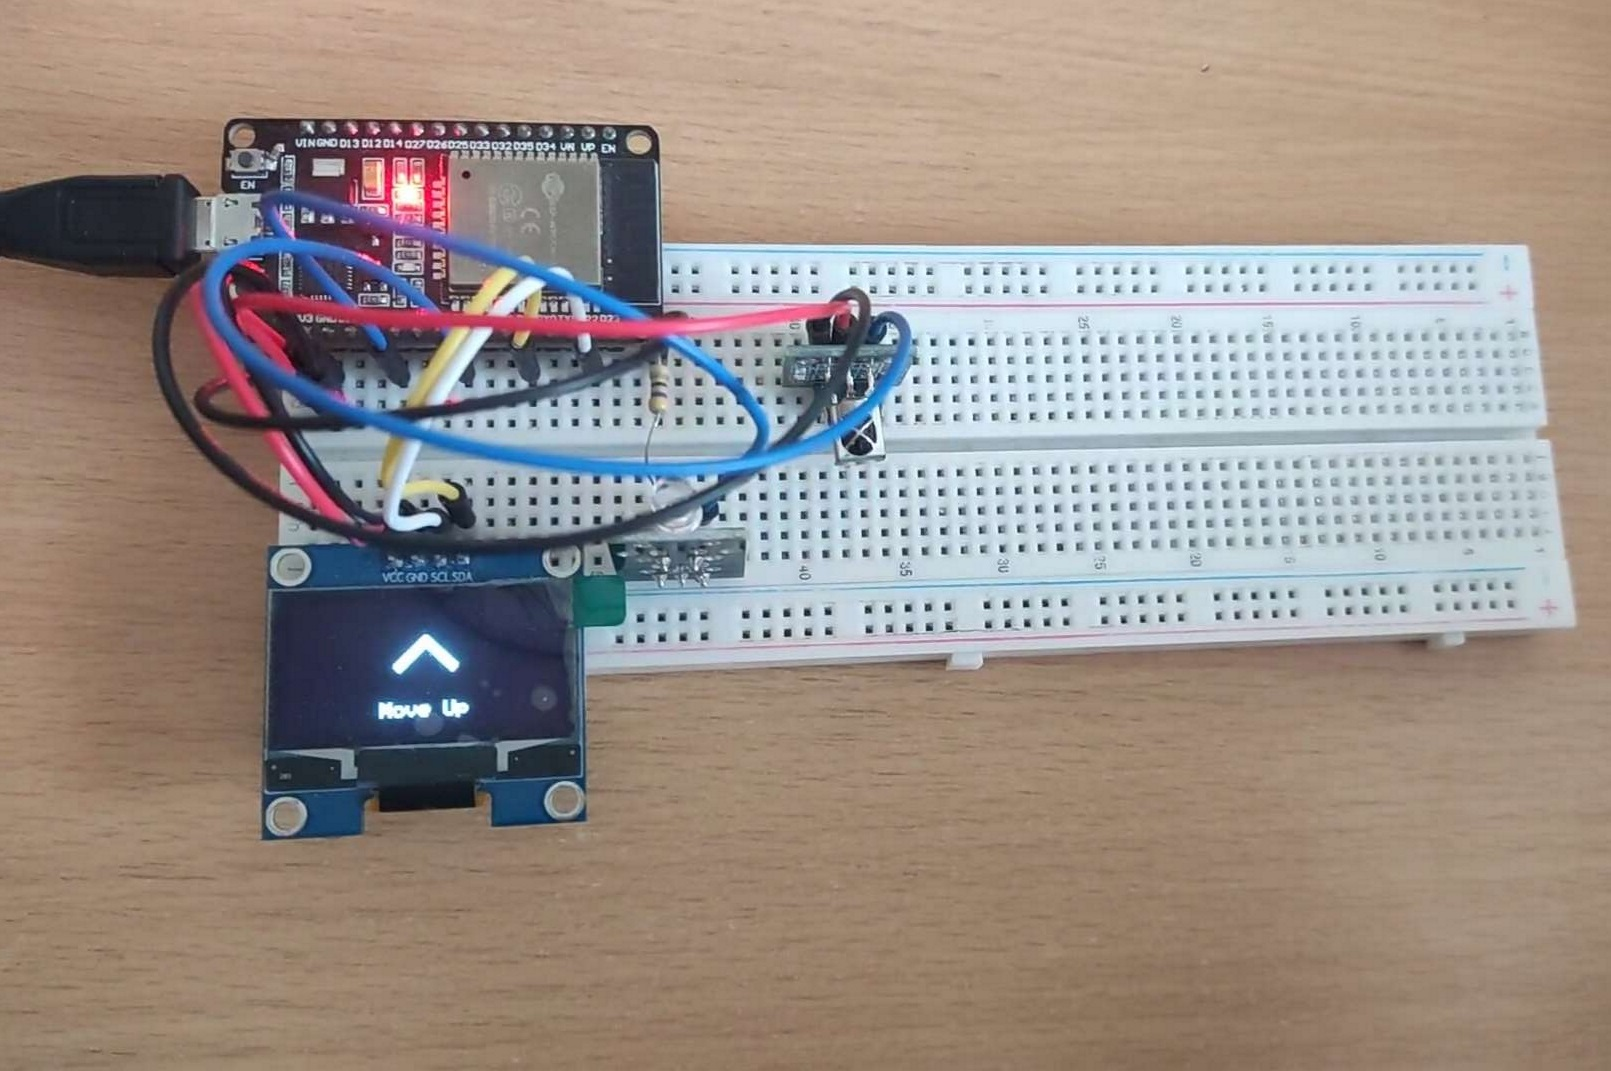
\includegraphics[width=14cm]{images/drawMoveUp.jpg}
   \caption{Wynik wywołania metody rysującej strzałkę w górę z opisem na wyświetlaczu}
   \label{Fig:drawMoveUp}
\end{figure}

\clearpage

\section{Zakończenie}

Niniejsza praca miała na celu zaproponowanie rozwiązania sterowania telewizorem z poziomu smartfona dzięki aplikacji mobilnej i urządzeniu pośredniczącym opartemu o mikrokontroler z niezbędnymi modułami. Omówiono w niej technologie i~koncepty, z których korzystano podczas procesu projektowania tego systemu. Opisane zostały też najważniejsze elementy fizycznej części projektu, oprogramowanie mikrokontrolera, zbudowana aplikacja mobilna oraz ich współpraca w cely sterowania telewizorem.

Utworzony prototyp systemu zapewnił możliwość programowania przycisków pilota w aplikacji mobilnej w oparciu o szesnastkowe kody sygnałów podczerwonych. Kody te można uzyskać przeglądając sieć i strony producentów urządzeń multimedialnych oraz dzięki wbudowanemu w urządzenie pośredniczące czytnikowi kodów IR, który po odebraniu takiego kodu przez podczerwień, wyświetla go na ekranie OLED. Przy pomocy serwera BLE zastosowanego na urządzeniu wysyłającym sygnały podczerwone zapewniono także dostęp do systemu dla wielu użytkowników jednocześnie. Utworzona aplikacja mobilna jest prosta w użytkowaniu i intuicyjna nawet dla użytkowników nieobytych z technologią obecną w dzisiejszych smartfonach, a duże i wyraziste elementy pozwalają się dostrzec nawet z większych odległości.

Zaprojektowany prototypowy system aplikacji mobilnej i urządzenia pośredniczącego opartego o mikrokontroler jest już w pełni funkcjonalny i może nawet zostać przekształcony do produktu komercyjnego. Aby zwiększyć jednak atrakcyjność tego rozwiązania na rynku, można wskazać kilka usprawnień jak na przykład:
\begin{itemize}[label=-,labelsep=0.4cm,leftmargin=0.65cm]
   \item zamknięcie urządzenia pośredniczącego w wygodnej prostokątnej obudowie z odpowiednim rozłożeniem modułów,
   \item wprowadznie automatyzacji programowania kodów IR i wczytywania ich z plików JSON, udostępnianych też na stronie internetowej firmy,
   \item dodanie obsługi inteligentnych gestów użytkownika w aplikacji dla konkretnych typów urządzeń,
   \item wprowadzenie kreatora ekranów przycisków pilota w aplikacji dla maksymalnej uniwersalności rozwiązania,
   \item wprowadzenie systemu logowania, aby przechowywać zestawy przycisków na serwerze, dzięki czemu będą one dostępne dla wielu urządzeń tego użytkownika
   
\end{itemize}

Autor za własny wkład pracy uważa: 
\begin{itemize}[label=-,labelsep=0.4cm,leftmargin=0.65cm]
   \item przegląd i dobór technologii do utworzonego rozwiązania,
   \item zaprojektowanie urządzenia pośredniczącego opartego o mikrokontroler wysyłającego i odbierającego sygnały IR,
   \item zaprojektowanie interfejsu użytkownika aplikacji mobilnej,
   \item zaprojektowanie komunikacji aplikacji mobilnej pilota uniwersalnego z mikrokontrolerem w oparciu o~technologię BLE,
   \item utworzenie odpowiedniego oprogramowania sterującego dla mikrokontrolera,
   \item zbudowanie i oprogramowanie aplikacji mobilnej,
   \item opis oprogramowania i przedstawienie elementów utworzonego systemu.
   
\end{itemize}

\clearpage
\addcontentsline{toc}{section}{Literatura}
\bibliography{biblgr}
\bibliographystyle{plain}

\clearpage

\makesummary

\end{document}
